\documentclass[12pt,letterpaper]{article}
\usepackage{fullpage}
\usepackage[top=2cm, bottom=4.5cm, left=2.5cm, right=2.5cm]{geometry}
\usepackage{amsmath,amsthm,amsfonts,amssymb,amscd}
\usepackage{lastpage}
\usepackage{enumerate}
\usepackage{fancyhdr}
\usepackage{mathrsfs}
\usepackage{xcolor}
\usepackage{graphicx}
\usepackage{listings}
\usepackage{hyperref}
\usepackage{booktabs}

\hypersetup{%
  colorlinks=true,
  linkcolor=blue,
  linkbordercolor={0 0 1}
}

\renewcommand\lstlistingname{Algorithm}
\renewcommand\lstlistlistingname{Algorithms}
\def\lstlistingautorefname{Alg.}

\lstdefinestyle{Python}{
    language        = Python,
    frame           = lines,
    basicstyle      = \footnotesize,
    keywordstyle    = \color{blue},
    stringstyle     = \color{green},
    commentstyle    = \color{red}\ttfamily
}

\setlength{\parindent}{0.0in}
\setlength{\parskip}{0.05in}

% Edit these as appropriate
\newcommand\course{Introdution to Machine Learning}
\newcommand\hwnumber{2}                  % <-- homework number
\newcommand\NetIDa{WangZhiyi, 922182514} % <-- NetID of person #1
\newcommand\NetIDb{ZhangTianyao, 922182332} % <-- NetID of person #2 (Comment this line out for problem sets)

\pagestyle{fancyplain}
\headheight 35pt
\lhead{\NetIDa}
\lhead{\NetIDa\\\NetIDb}                 % <-- Comment this line out for problem sets (make sure you are person #1)
\chead{\textbf{\Large Homework \hwnumber}}
\rhead{\course \\ \today}
\lfoot{}
\cfoot{}
\rfoot{\small\thepage}
\headsep 1.5em

\begin{document}


\section*{Question 1}

\subsection*{Que (a)}
\begin{equation}
	\because A^TA=I
\end{equation}
So, $A$ is a reversible matrix.
\begin{equation}
	\Sigma_x=\frac1n\sum^6_{i=1}x_ix_i^T
\end{equation}
Among this equation,
\begin{eqnarray}
	x_ix_i^T
	&=& Az_i(Az_i)^T\\
	&=& Az_iz_i^TA^T\nonumber\\
	&=& A(z_iz_i^T)A^T\nonumber\\
	&=& AA^T\nonumber
\end{eqnarray}
So that, the equation can be simplified to
\begin{eqnarray}
	\Sigma_x
	&=& \frac1n\sum^6_{i=1}AA^T\\
	&=& A\frac1n\sum^6_{i=1}A^T\nonumber
\end{eqnarray}
Then, compute the eigenvalue(s) of $\Sigma_z$
\begin{eqnarray}
	|\lambda E-\Sigma_z|
	&=& \left|\begin{array}{cccc}
		\lambda-3 & 0 & 0 & 0 \\
		0 & \lambda-21 & 0 & 0 \\
		0 & 0 & \lambda-13 & -8 \\
		0 & 0 & -8 & \lambda-13
	\end{array}\right|\\
	&=& (\lambda-3)(\lambda-21)[(\lambda-13)^2-(-8)^2]\nonumber\\
	&=& (\lambda-3)(\lambda-21)(\lambda-21)(\lambda-5)\nonumber\\
	&=&0\nonumber
\end{eqnarray}
Solve it, we can get that
\begin{equation}
	\lambda_1=3,
	\lambda_2=21,
	\lambda_3=21,
	\lambda_4=5
\end{equation}
However, $A\in\mathbb{R}^{6\times 4}$, so we need to transform $\Sigma_x$ and $\lambda_x$
\begin{eqnarray}
	\Sigma_x
	&=& AV\Lambda V^TA^T\\
	&=& (AV)\Lambda (AV)^T\nonumber
\end{eqnarray}
Let's expand $(AV)$ to $\mathbb{R}^6$, so that
\begin{equation}
	\lambda_1=3,
	\lambda_2=21,
	\lambda_3=21,
	\lambda_4=5,
	\lambda_5=0,
	\lambda_6=0
\end{equation}
Then, compute the sum of eigenvalues
\begin{eqnarray}
	S_\lambda
	&=& Tr(\Sigma_x)\\
	&=& Tr(A\Sigma_zA^T)\nonumber\\
	&=& Tr((AA^T)\Sigma_z)\nonumber\\
	&=& Tr(\Sigma_z)\nonumber\\
	&=& 3+21+21+5+0+0\nonumber\\
	&=& 50\nonumber
\end{eqnarray}

\subsection*{Que (b)}
First, compute the estimated value of mean reconstruction error
\begin{eqnarray}
	error(d)
	&=& \frac1N\sum^N_{i=1}||x_i-\tilde{x}_i||^2_2\\
	&=& \sum^D_{i=d+1}\lambda_i\nonumber\\
	&<& \frac{50}4=17.5\nonumber
\end{eqnarray}
It means that
\begin{equation}
	\lambda_1+\lambda_2+\cdots+\lambda_d\geq37.5
\end{equation}
Meanwhile, sum of the top $d$ values shows that
\begin{equation}
\begin{cases}
	\max\lambda_1=21<37.5\\
	\max\lambda_1+\max\lambda_2=21+21=42>37.5
\end{cases}
\end{equation}
In conclusion, the value of PCA direction must be \textbf{not less than $2$}

\subsection*{Que (c)}
As the solving process in \textbf{Q-a} and \textbf{Q-b} above, compute the new $y$
\begin{equation}
	x\sim\mathcal{N}(0,\Sigma_x),v\sim\mathcal{N}(0,\Sigma_v)
\end{equation}
And $x$ is independent of $v$, so that
\begin{equation}
	y\triangleq x+v\in\mathcal{N}(0+0,\Sigma_x+\Sigma_v)=\mathcal{N}(0,\Sigma_x+\Sigma_v)
\end{equation}
Then compute $\Sigma_y$
\begin{eqnarray}
	\Sigma_y
	&=& \Sigma_x'+\Sigma_z\\
	&=& \left[\begin{array}{cccc}
		3 & 0 & 0 & 0\\
		0 & 21 & 0 & 0\\
		0 & 0 & 13 & 8\\
		0 & 0 & 8 & 13
	\end{array}\right]'+\left[\begin{array}{cccccc}
		5 & 0 & 0 & 0 & 0 & 0\\
		0 & 5 & 0 & 0 & 0 & 0\\
		0 & 0 & 5 & 0 & 0 & 0\\
		0 & 0 & 0 & 5 & 0 & 0\\
		0 & 0 & 0 & 0 & 5 & 0\\
		0 & 0 & 0 & 0 & 0 & 5
	\end{array}\right]\nonumber\\
	&=& \left[\begin{array}{cccccc}
		3 & 0 & 0 & 0 & 0 & 0\\
		0 & 21 & 0 & 0 & 0 & 0\\
		0 & 0 & 13 & 8 & 0 & 0\\
		0 & 0 & 8 & 13 & 0 & 0\\
		0 & 0 & 0 & 0 & 0 & 0\\
		0 & 0 & 0 & 0 & 0 & 0
	\end{array}\right]+\left[\begin{array}{cccccc}
		5 & 0 & 0 & 0 & 0 & 0\\
		0 & 5 & 0 & 0 & 0 & 0\\
		0 & 0 & 5 & 0 & 0 & 0\\
		0 & 0 & 0 & 5 & 0 & 0\\
		0 & 0 & 0 & 0 & 5 & 0\\
		0 & 0 & 0 & 0 & 0 & 5
	\end{array}\right]\nonumber\\
	&=& \left[\begin{array}{cccccc}
		8 & 0 & 0 & 0 & 0 & 0\\
		0 & 26 & 0 & 0 & 0 & 0\\
		0 & 0 & 18 & 8 & 0 & 0\\
		0 & 0 & 8 & 18 & 0 & 0\\
		0 & 0 & 0 & 0 & 5 & 0\\
		0 & 0 & 0 & 0 & 0 & 5
	\end{array}\right]\nonumber
\end{eqnarray}

\begin{eqnarray}
	|\lambda E-\Sigma_y|
	&=& \left|\begin{array}{cccccc}
		\lambda'-8 & 0 & 0 & 0 & 0 & 0\\
		0 & \lambda'-26 & 0 & 0 & 0 & 0\\
		0 & 0 & \lambda'-18 & -8 & 0 & 0\\
		0 & 0 & -8 & \lambda'-18 & 0 & 0\\
		0 & 0 & 0 & 0 & \lambda'-5 & 0\\
		0 & 0 & 0 & 0 & 0 & \lambda'-5
	\end{array}\right|\nonumber\\
	&=& (\lambda'-8)(\lambda'-26)[(\lambda'-18)-(-8)^2](\lambda'-5)(\lambda'-5)\nonumber\\
	&=& (\lambda'-8)(\lambda'-26)(\lambda'-26)-(\lambda'-10)(\lambda'-5)(\lambda'-5)\nonumber\\
	&=& 0\nonumber
\end{eqnarray}
Solve it, and we get that
\begin{equation}
	\lambda_1'=8,
	\lambda_2'=26,
	\lambda_3'=26,
	\lambda_4'=10,
	\lambda_5'=5,
	\lambda_6'=5
\end{equation}
Then compute the sum of eigenvalues
\begin{eqnarray}
	S_{\lambda'}
	&=& \sum^6_{i=1}\lambda'_i\\
	&=& 8+26+26+10+5+5\nonumber\\
	&=& 80\nonumber
\end{eqnarray}
\begin{eqnarray}
	error'(d)
	&=& \sum^D_{i=d+1}\lambda'_i\\
	&<& \frac{80}4=20\nonumber
\end{eqnarray}
\begin{equation}
	\lambda'_1+\lambda'_2+\cdots+\lambda'_d\geq 60
\end{equation}
Meanwhile, sum of the top d values shows that
\begin{equation}
\begin{cases}
	\max\lambda'_1+\max\lambda'_2=26+26=52<60
	\max\lambda'_1+\max\lambda'_2+\max\lambda'_3=26+26+10=62>60
\end{cases}
\end{equation}
In conclusion, the new value of PCA direction must be \textbf{not less than $3$}


\section*{Question 2}
We consider two situations of the questions.
\subsection*{1. a>1}
\subsubsection*{First iteration}We choose $x_1$ and $x_4$ as fixed points. Then calculate the distance between each pair of fixed point and the unfixed point.
\par Assume that the fixed point is $p_i=(x_i,y_i)$, unfixed point is $p_j=(x_j,y_j)$ The distance($d_{ij}$) between them can be calculated by equation\ref{q2e1}:
\begin{equation}\label{q2e1}
  d_{ij}=\sqrt{\left( x_i-x_j \right) ^2+\left( y_i-y_j \right) ^2}
\end{equation}
{\bf Group Result: }The iteration result is shown in table \ref{first iteration}. The group result is follows, $G_{ij}$ is respect for the $j$ group in $i$ iteration.
 %Table generated by Excel2LaTeX from sheet 'Sheet2'
\begin{table}[!htbp]
  \centering
  \caption{First iteration}
    \begin{tabular}{|c|c|c|}
   \toprule
            & $x_1$    & $x_4$ \\
    \hline
    $x_2$    & \textcolor[rgb]{1.000, 0.000, 0.000}{1}     & $\sqrt{a^2+1}$ \\
    \hline
    $x_3$    & $\sqrt{a^2+1}$     & \textcolor[rgb]{1.000, 0.000, 0.000}{1} \\
    \bottomrule
    \end{tabular}%
  \label{first iteration}%
\end{table}%

\begin{equation}\label{q2e2}
  Result_1: x_1,x_2\in G_{11}, x_3,x_4\in G_{12}
\end{equation}
Then generate another group of fixed points of a new group, $p_i=\left( x_i,y_i \right) \in P$. All fixed points of a iteration belong to the set $P$. $x_i$ and $y_i$ is calculated by equation \ref{q2e3}.$X,Y$ are the coordinates of the points belong to the same group.
\begin{equation}\label{q2e3}
  x_i=\bar{X}, y_i=\bar{Y}
\end{equation}
The result is $p_1(0,\frac{1}{2})$, $p_2(a,\frac{1}{2})$
\newpage
\subsubsection*{Second iteration}Then we choose the $p_1$ and $p_2$ as fixed points. Then calculate the distance between fixed point and sample point.
% Table generated by Excel2LaTeX from sheet 'Sheet3'
\begin{table}[htbp]
  \centering
  \caption{Second iteration}
    \begin{tabular}{|c|c|c|}
    \toprule
          & $p_1$ &$p_2$ \\
    \hline
    $x_1$    &  \textcolor[rgb]{1.000, 0.000, 0.000}{$\frac{1}{2}$}     & $\sqrt{a^2+\frac{1}{4}}$ \\
    \hline
    $x_2$    &  \textcolor[rgb]{1.000, 0.000, 0.000}{$\frac{1}{2}$}      & $\sqrt{a^2+\frac{1}{4}}$ \\
    \hline
    $x_3$    &   $\sqrt{a^2+\frac{1}{4}}$    & \textcolor[rgb]{1.000, 0.000, 0.000}{$\frac{1}{2}$}  \\
    \hline
    $x_4$    &  $\sqrt{a^2+\frac{1}{4}}$     & \textcolor[rgb]{1.000, 0.000, 0.000}{$\frac{1}{2}$}  \\
    \bottomrule
    \end{tabular}%
  \label{Second iteration}%
\end{table}%
\newline
{\bf Result: }According to K-Means, the result is:
\begin{equation}\label{q2eq5}
  Result_2: x_1,x_2\in G_{21}, x_3,x_4\in G_{22}
\end{equation}
Therefore, we can get $Result_1=Result_2$, in others words, the K-Means algorithm has converged.
\section*{2. a<1}
We choose $x_1$ and $x_2$ as the initial fixed points.
\subsection*{First iteration}
First iteration result is shown in table \ref{q2tb3}
% Table generated by Excel2LaTeX from sheet 'Sheet3'
\begin{table}[htbp]
  \centering
  \caption{First iteration}
    \begin{tabular}{|c|c|c|}
    \toprule
          & $x_1$    & $x_2$ \\
    \hline
    $x_3$    & $\sqrt{a^2+1}$     & \textcolor[rgb]{1.000, 0.000, 0.000}{$a$} \\
    \hline
    $x_4$    & \textcolor[rgb]{1.000, 0.000, 0.000}{$a$}     & $\sqrt{a^2+1}$ \\
    \bottomrule
    \end{tabular}%
  \label{q2tb3}%
\end{table}%
\subsubsection*{Group Result}The group result is
\begin{equation}\label{q2eq5}
  Result_1: x_1, x_4\in G_{11}, x_2, x_3\in G_{12}
\end{equation}
Similar to the $a>1$ condition, we choose $p_1=(\frac{a}{2},1), p_2=(\frac{a}{2},0)$ as fixed points
\newpage
\subsection*{Second iteration}
Apply K-Means to the points, we get the iteration result:
% Table generated by Excel2LaTeX from sheet 'Sheet3'
\begin{table}[!htbp]
  \centering
  \caption{Secondly iteration}
    \begin{tabular}{|c|c|c|}
    \toprule
          & $p_1$    & $p_2$ \\
    \hline
    $x_1$    & \textcolor[rgb]{1.000, 0.000, 0.000}{$\frac{a}{2}$}     & $\sqrt{\frac{a^2}{4}+1}$ \\
    \hline
    $x_2$    &   $\sqrt{\frac{a^2}{4}+1}$   & \textcolor[rgb]{1.000, 0.000, 0.000}{$\frac{a}{2}$}  \\
    \hline
    $x_3$    & $\sqrt{\frac{a^2}{4}+1}$      & \textcolor[rgb]{1.000, 0.000, 0.000}{$\frac{a}{2}$}  \\
    \hline
    $x_4$    & \textcolor[rgb]{1.000, 0.000, 0.000}{$\frac{a}{2}$}       & $\sqrt{\frac{a^2}{4}+1}$ \\
    \bottomrule
    \end{tabular}%
  \label{tab:addlabel}%
\end{table}%
\subsubsection*{Group Result}The group result is
\begin{equation}\label{q2eq5}
  Result_2: x_1, x_4\in G_{21}, x_2, x_3\in G_{22}
\end{equation}
Therefore, $Result_1=Reuslt_2$, in others words, the K-Means algorithm has converged.
\section*{3. a=1}
If $a=1$ we can divide the four points into ${x_1, x_2}$ and ${x_3, x_4}$ or we can also divide them into ${x_1, x_3}$ and ${x_2, x_4}$

\section*{Question 3}

It has several options.

\begin{equation}
	\mu_x=\frac1N\sum^N_{i=1}x_i\triangleq\bar{x},\Sigma_x=\frac1N\sum^N_{i=1}(x_i-\mu_x)(x_i-\mu_x)^T
\end{equation}

\subsubsection*{Option 1}
\begin{equation}
	\mu_1(1,0),\mu_2(10^5,0)
\end{equation}
So that $\mu_1$ has all the points while $\mu_2$ has none.

\subsubsection*{Option 2}
\begin{equation}
	\mu_1(-1,0),\mu_2(2,0)
\end{equation}
So that $mu_1$ has the left point and the middle circle while $mu_2$ has the right circle.

\subsubsection*{Conclusion}
Because of this, the \textbf{Option 1} attains a lower value of the objective function.



\section*{Question 4}
There are two rules of PLA:
\par{\bf First rule:} The best $W$ is exist.
\begin{equation}\label{q4eq1}
  \exists w_i\in W_f, \forall x_i\in X_n,\\
  s.t. y_i=sign(W_f^Tx_i)
\end{equation}
\par{\bf Second rule:} Only if the clustering result is not correct, the $W$ will be updated.
\begin{equation}\label{q4eq2}
  y_{n\left( t \right)}W_t^TX_{n\left( t \right)}\leqslant 0
\end{equation}
In every iteration, $y_{n\left( t \right)}W_t^TX_{n\left( t \right)}\geqslant \underset{n}{\min}y_nW_f^TX_n>0$. Then we use $W_{f}^{T}\cdot W_t$ to measure the similarity between $W_f$ and $W_t$
\begin{eqnarray}\label{q4eq3}
% \nonumber % Remove numbering (before each equation)
  W_{f}^{T}\cdot W_t
  &=& W_{f}^{T}\\
  &=& W_{f}(W_(t-1)+\lambda(d_t-y_t)X_t\nonumber\\
  &\geqslant & W_{f}^{T}\cdot W_0+t\underset{n}{\min}y_nW_f^TX_n\nonumber\\
  &=& \underset{n}{\min}y_nW_f^TX_n \nonumber
\end{eqnarray}
Then we should distinguish the update direction:
\begin{eqnarray}
% \nonumber % Remove numbering (before each equation)
\lVert W_{t+1} \rVert ^2
    &=&\lVert W_t+y_nX_n \rVert ^2\\
    &=&\lVert W_t \rVert ^2+2y_nW_t^TX_n+\lVert y_nX_n \rVert ^2\nonumber\\
    &\leqslant& \lVert W_t \rVert ^2+\lVert y_nX_n \rVert ^2\nonumber\\
    &\leqslant& \lVert W_t \rVert ^2+\underset{n}{\max}\lVert y_nX_n \rVert ^2\nonumber\\
    &\leqslant& \lVert W_0 \rVert ^2+\underset{n}{T\cdot \max}\lVert y_nX_n \rVert ^2\nonumber
\end{eqnarray}
% Table generated by Excel2LaTeX from sheet 'Sheet2'
Finally, we assume that $T$ is the time of iterations.
\begin{eqnarray}
% \nonumber % Remove numbering (before each equation)
    \frac{W_{f}^{T}}{\lVert W_{f}^{T} \rVert}\frac{W_T}{\lVert W_T \rVert}
    &=& \frac{T\cdot \underset{n}{\min}y_nW_f^TX_n}{\lVert W_{f}^{T} \rVert \lVert W_T \rVert}\\
    &\geqslant& \frac{T\cdot \underset{n}{\min}y_nW_f^TX_n}{\lVert W_{f}^{T} \rVert \underset{n}{\sqrt{T}\cdot \max}\lVert y_nX_n \rVert ^2}\nonumber\\
    &\geqslant& \frac{\sqrt{T}\cdot \underset{n}{\min}y_nW_f^TX_n}{\lVert W_{f}^{T} \rVert \underset{n}{\cdot \max}\lVert y_nX_n \rVert ^2}\nonumber\\
    &\because& \frac{W_{f}^{T}}{\lVert W_{f}^{T} \rVert}\frac{W_T}{\lVert W_T \rVert}\leqslant \cos \left( \left< W_f,W_T \right> \right) \leqslant 1\nonumber\\
    &\therefore& \sqrt{T}\leqslant \frac{\lVert W_{f}^{T} \rVert \underset{n}{\cdot \max}\lVert y_nX_n \rVert ^2}{\underset{n}{\min}y_nW_f^TX_n}\nonumber\\
    &\therefore& T\leqslant \left( \frac{\lVert W_{f}^{T} \rVert \underset{n}{\cdot \max}\lVert y_nX_n \rVert ^2}{\underset{n}{\min}y_nW_f^TX_n} \right) ^2\nonumber
\end{eqnarray}



%Answer to the problem goes here.
%
%\begin{enumerate}
%  \item
%   Problem 1 part 1 answer here.
%  \item
%    Problem 1 part 2 answer here.
%
%    Here is an example typesetting mathematics in \LaTeX
%\begin{equation*}
%    X(m,n) = \left\{\begin{array}{lr}
%        x(n), & \text{for } 0\leq n\leq 1\\
%        \frac{x(n-1)}{2}, & \text{for } 0\leq n\leq 1\\
%        \log_2 \left\lceil n \right\rceil \qquad & \text{for } 0\leq n\leq 1
%        \end{array}\right\} = xy
%\end{equation*}
%
%    \item Problem 1 part 3 answer here.
%
%    Here is an example of how you can typeset algorithms.
%    There are many packages to do this in \LaTeX.
%
%    \lstset{caption={Caption for code}}
%    \lstset{label={lst:alg1}}
%    \begin{lstlisting}[style = Python]
%    from package import Class # Mesh required for..
%
%    cinstance = Class.from_obj('class.obj')
%    cinstance.go()
%    \end{lstlisting}
%
%  \item Problem 1 part 4 answer here.
%
%    Here is an example of how you can insert a figure.
%    \begin{figure}[!h]
%    \centering
%    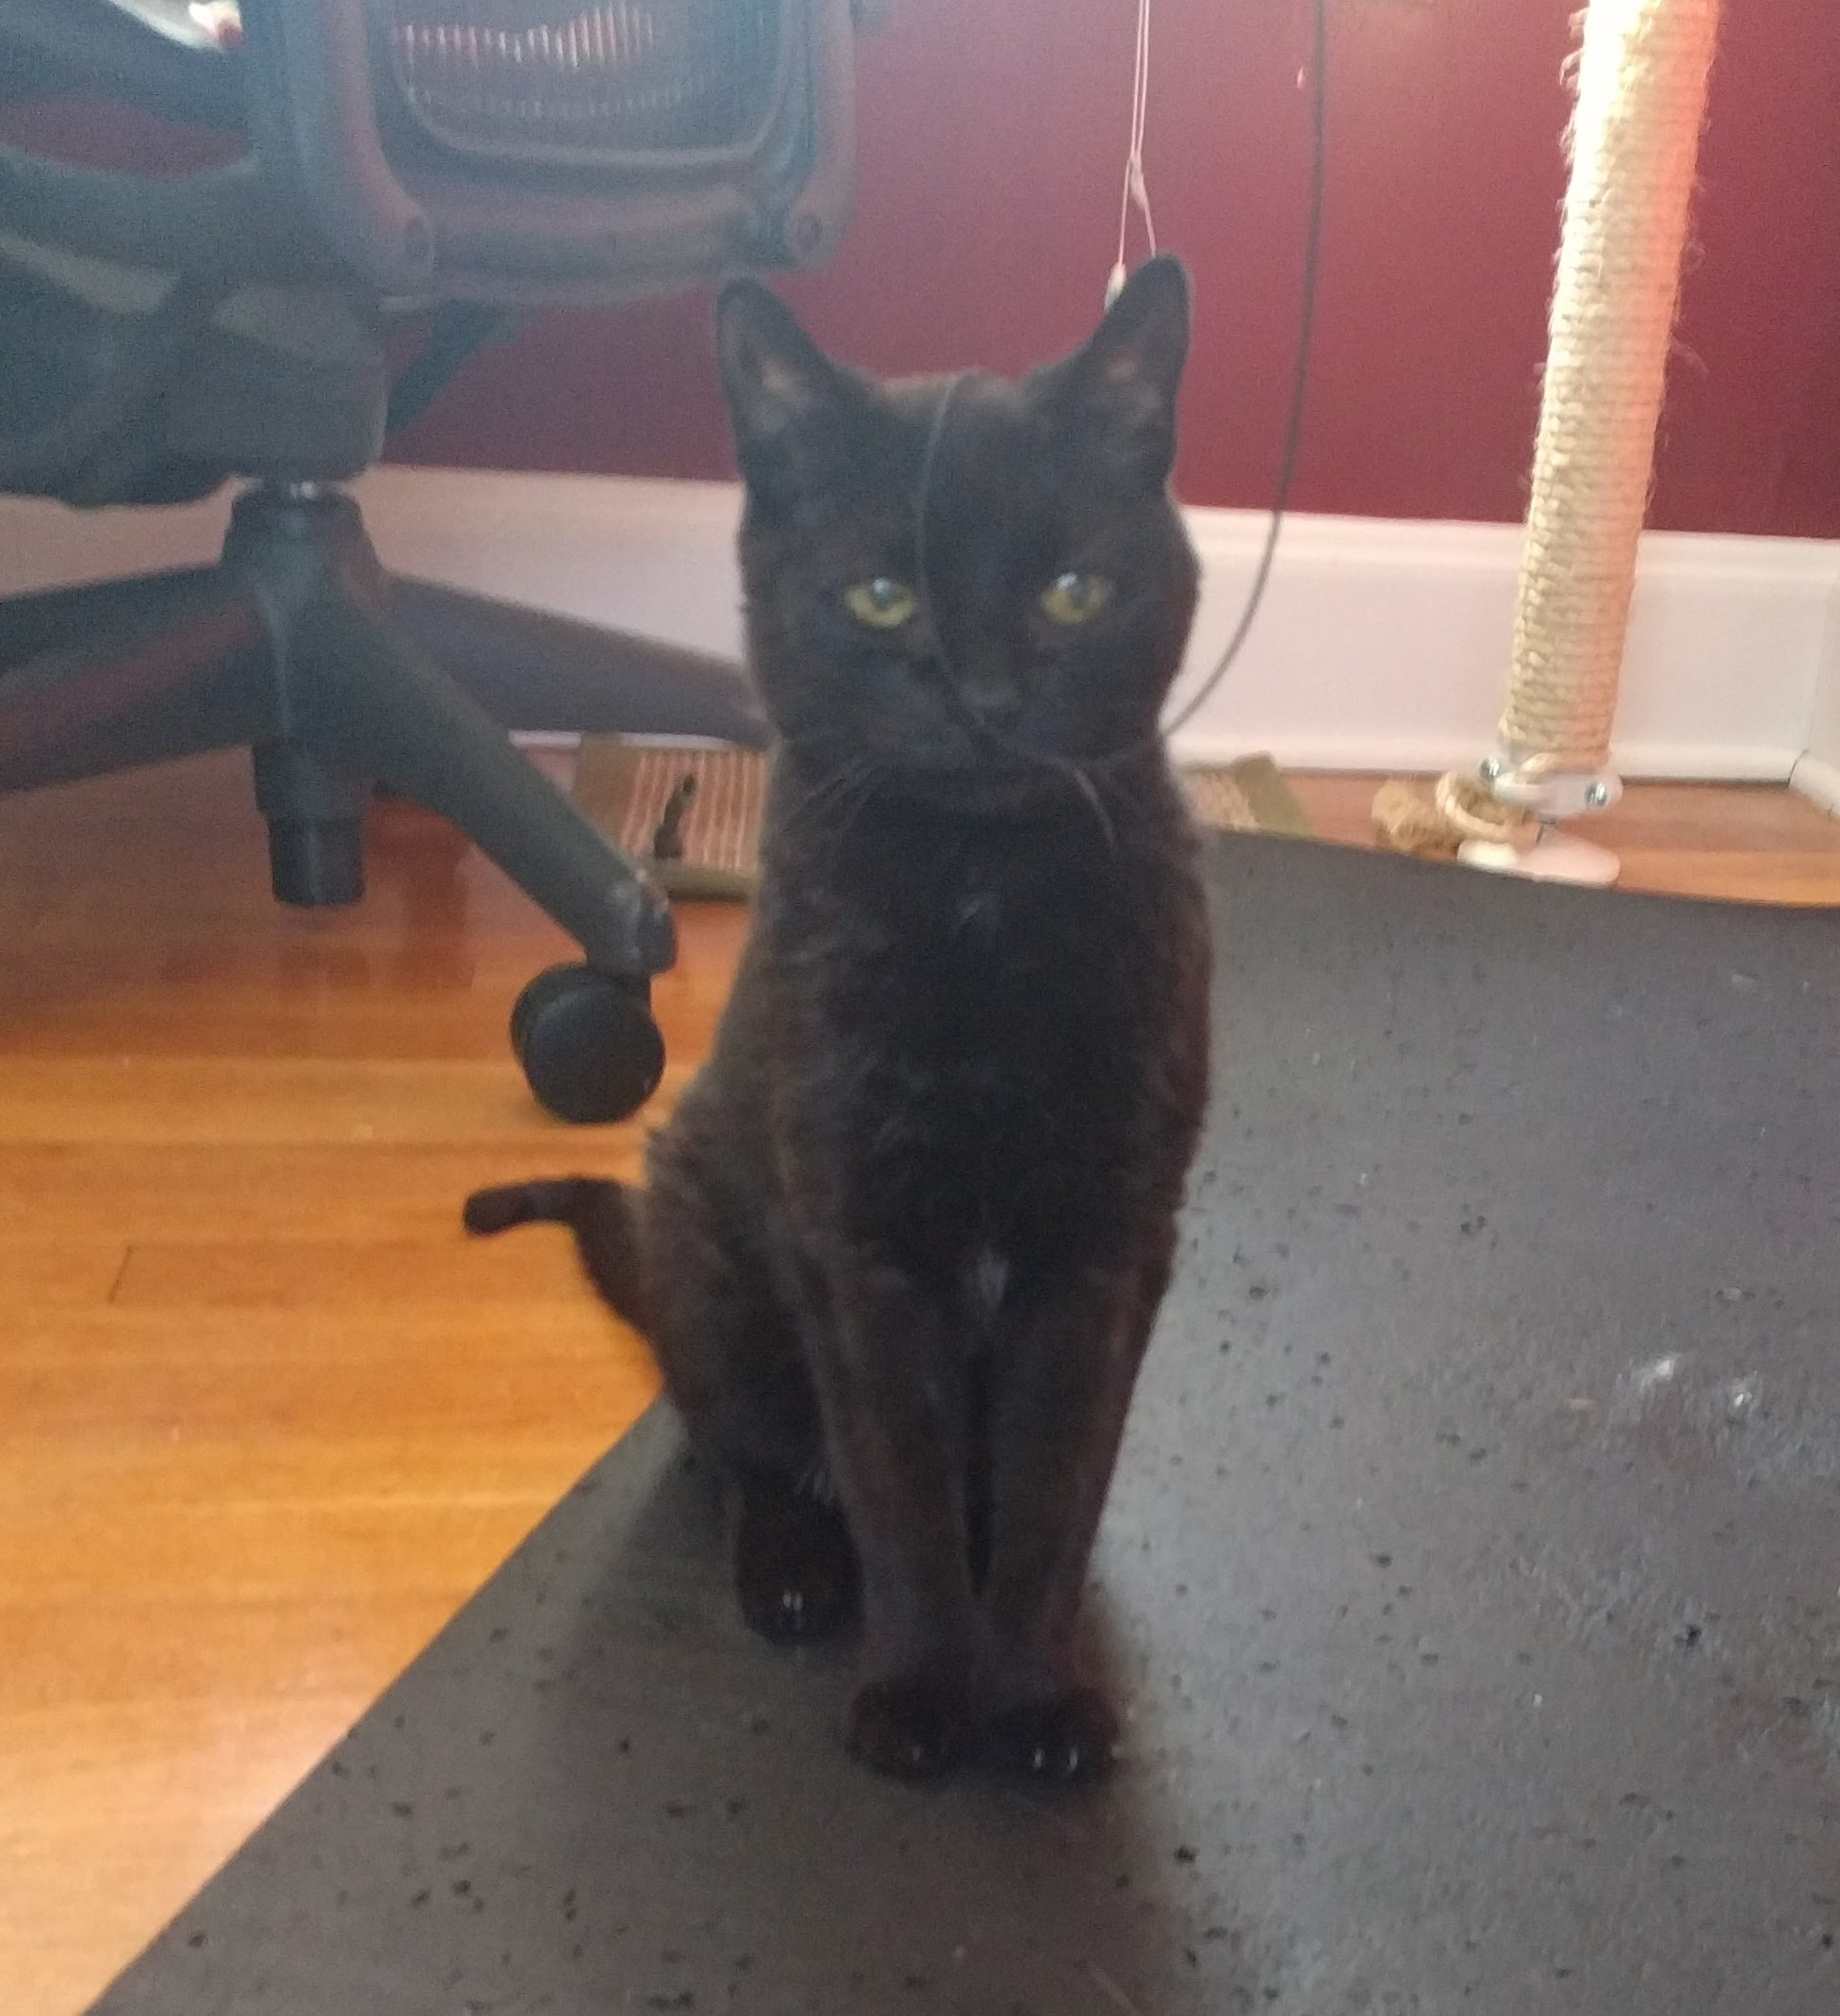
\includegraphics[width=0.3\linewidth]{heidi.jpg}
%    \caption{Heidi attacked by a string.}
%    \end{figure}
%\end{enumerate}






\end{document}
